% \documentclass[handout]{beamer} %"handout" serveix per a treure els \pause
\documentclass{beamer} %"handout" serveix per a treure els \pause
\usepackage{preamble}

\usetheme{Copenhagen}
\usecolortheme{seahorse}

% \addbibresource{references.bib}

%gets rid of bottom navigation bars
\setbeamertemplate{footline}[frame number]{}

%gets rid of bottom navigation symbols
\setbeamertemplate{navigation symbols}{}

%gets rid of footer
%will override 'frame number' instruction above
%comment out to revert to previous/default definitions
\setbeamertemplate{headline}{}
\setbeamertemplate{footline}{}
% Remove the "Figure" prefix from captions
\captionsetup[figure]{labelformat=empty}
% \setbeameroption{show notes}

\newtheorem{thm}[theorem]{Teorema}

\title{Propagació numèrica d'errors\\dels satè\lgem its en òrbita terrestre}
\author{Víctor Ballester\texorpdfstring{\vspace{0.15cm}\\}{}{\small Supervisor: Josep Maria Mondelo}}
\institute{Departament de Matemàtiques\\Facultat de Ciències}
\titlegraphic{
\includegraphics[width=0.3\textwidth]{../Images/uab.pdf}}
\date{11 de juliol de 2023}

\begin{document}
\selectlanguage{catalan}
\frame{\titlepage}
% add index
\begin{frame}{Motivació}
  \begin{itemize}
    \item Aproximadament 27\,000 satè\lgem its (actius i inactius) orbiten al voltant de la Terra.
    \item Diverses co\lgem isions involuntàries s'han produït en el passat.
    \item El model que considera la Terra com a massa puntual no és suficient. Necessitem un model més precís.
  \end{itemize}
  \vspace{0.5cm}\pause
  \textbf{Objectius:}
  \begin{itemize}
    \item Desenvolupar un model per al potencial de la Terra.
    \item Predir la posició de satè\lgem its considerant diverses pertorbacions.
    \item Estimar l'error de la trajectòria del satè\lgem it.
  \end{itemize}
\end{frame}
\begin{frame}{Índex}
  \tableofcontents
\end{frame}
\section{Equació per al geopotencial}
\begin{frame}{Equació per al geopotencial}
  \begin{minipage}{0.68\textwidth}
    Sigui $\Omega\subseteq \RR^3$ la regió que ocupa la Terra.
    \begin{gather*}
      \vf{g} = -\int_\Omega G\frac{\vf{r}-\vf{s}}{\norm{\vf{r}-\vf{s}}^3}\rho(\vf{s})\dd^3\vf{s}=\grad V\\
      V=\int_\Omega G\frac{\rho(\vf{s})}{\norm{\vf{r}-\vf{s}}}\dd^3\vf{s}
    \end{gather*}
  \end{minipage}\hfill
  \begin{minipage}{0.31\textwidth}
    \begin{figure}
      \centering
      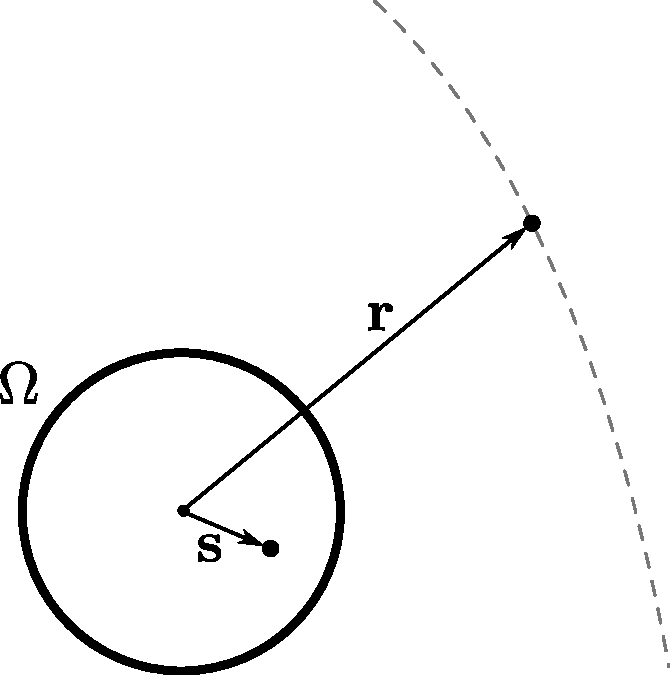
\includegraphics[width=\textwidth]{../Images/earth_pot.pdf}
    \end{figure}
  \end{minipage}
  \pause
  \begin{thm}
    $V$ satisfà el següent problema de valors de frontera exterior:
    \begin{equation*}\label{eq:dirichletProblem}
      \begin{cases}
        \laplacian V = 0 & \text{a } \Omega^c    \\
        V = f            & \text{a } \Fr{\Omega} \\
        \displaystyle\lim_{\norm{\vf{r}}\to\infty}V=0
      \end{cases}
    \end{equation*}
    on $f:\Fr{\Omega}\to\RR$ és el potencial gravitatori a la superfície de la Terra.
  \end{thm}
\end{frame}
\begin{frame}
  Buscant la solució explícita fent separació de variables, trobem que
  \begin{equation*}
    V =\frac{GM_\oplus}{R_\oplus}\sum_{n=0}^\infty \sum_{m=0}^n{\left(\frac{{R_\oplus}}{r}\right)}^{n+1}(\bar{C}_{n,m}Y_{n,m}^{\mathrm{c}}(\theta,\phi)+\bar{S}_{n,m}Y_{n,m}^{\mathrm{s}}(\theta,\phi))
  \end{equation*}
  on
  \begin{align*}
    Y_{n,m}^{\mathrm{c}}(\theta,\phi) & =N_{n,m}P_{n,m}(\cos\theta)\cos(m\phi) \\
    Y_{n,m}^{\mathrm{s}}(\theta,\phi) & =N_{n,m}P_{n,m}(\cos\theta)\sin(m\phi)
  \end{align*}
  són els \textbf{harmònics esfèrics}.
  \begin{figure}
    \centering
    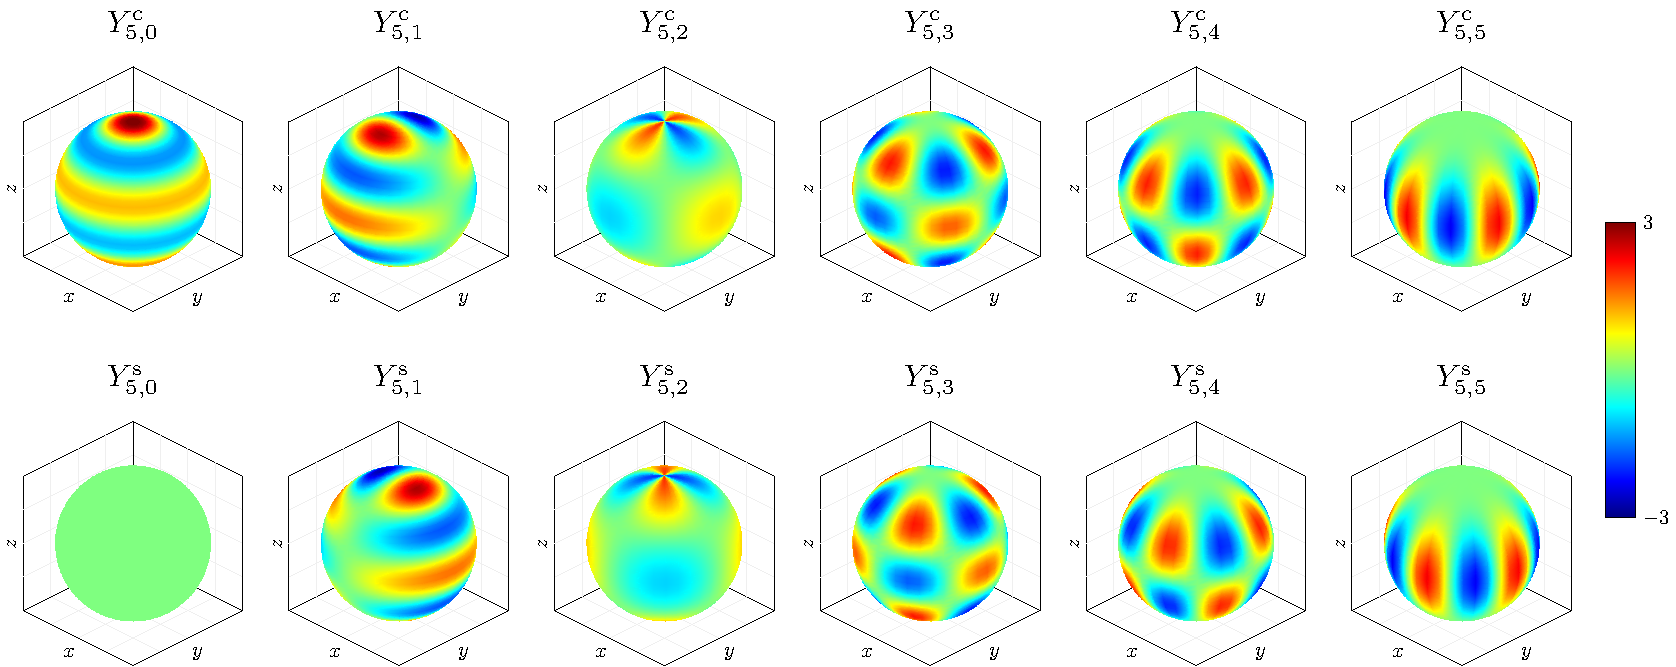
\includegraphics[width=\textwidth]{../Images/sphericalHarmonics.pdf}
  \end{figure}
\end{frame}
\section{Desviacions de l'eix de rotació de la Terra}
\begin{frame}{Desviacions de l'eix de rotació de la Terra}
  \begin{minipage}{0.49\textwidth}
    \begin{figure}
      \centering
      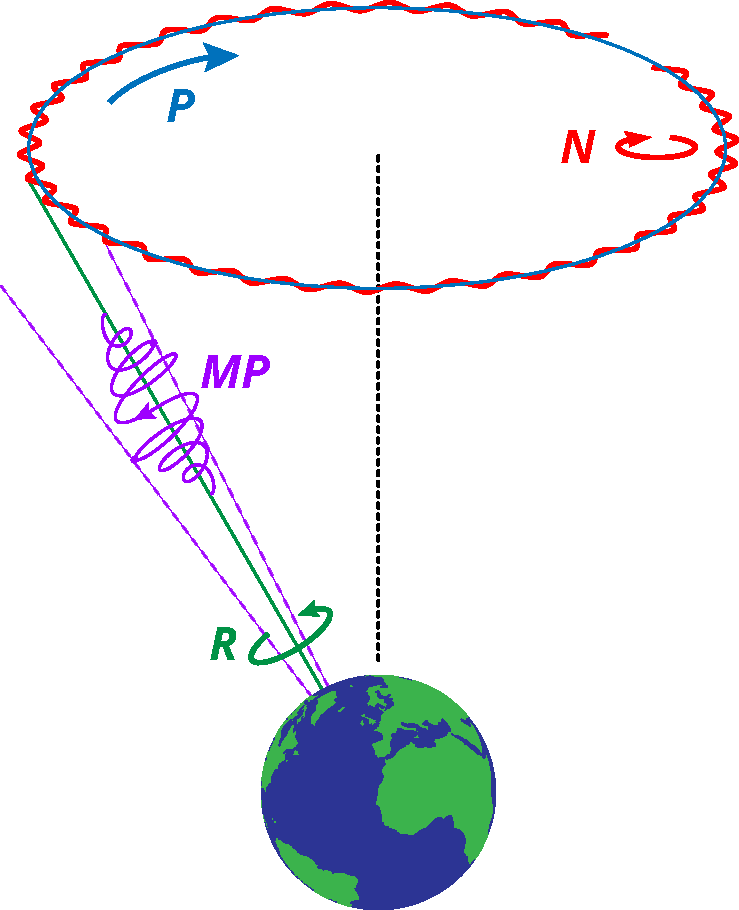
\includegraphics[width=\textwidth]{../Images/precession_nutation_ca.pdf}
    \end{figure}
  \end{minipage}
  \begin{minipage}{0.49\textwidth}
    \begin{itemize}
      \item \textcolor[RGB]{0,113,188}{{Precessió}}
      \item \textcolor[RGB]{255,0,0}{{Nutació}}
      \item \textcolor[RGB]{158,0,255}{{Moviment polar}}
      \item \textcolor[RGB]{0,146,70}{{Rotació}}
    \end{itemize}
    \vspace{1cm}
    \begin{figure}
      \centering
      \href{https://youtu.be/KnPk2T_kpco}{
        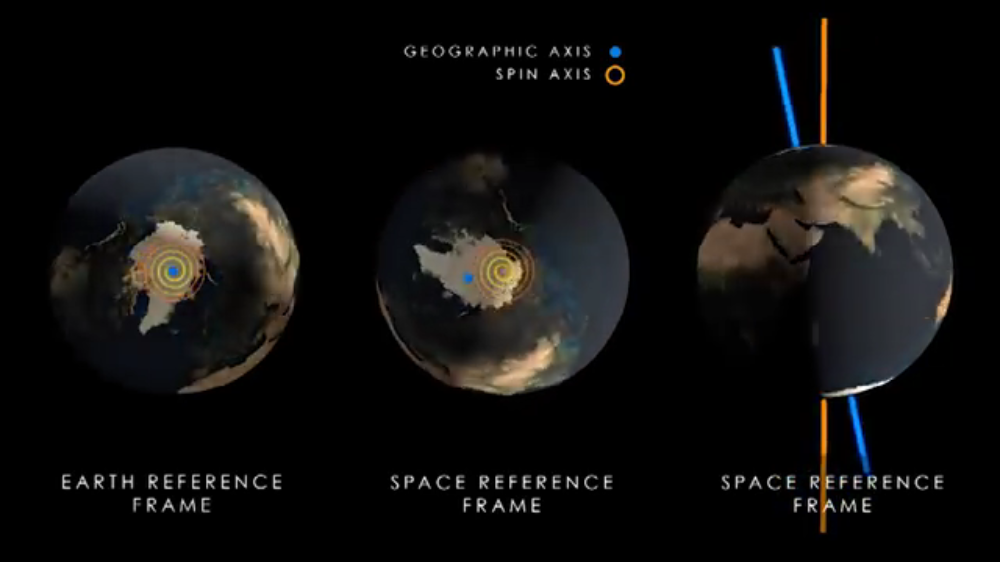
\includegraphics[width=\textwidth, keepaspectratio]{../Images/polarMotion_video_frame.png}
      }
      \vspace{-0.5cm}
      \caption{\tiny Font: \href{https://svs.gsfc.nasa.gov/20196}{NASA Earth Orientation Animations}}
    \end{figure}
  \end{minipage}
\end{frame}
% \begin{frame}{Transformació entre sistemes}

% \begin{figure}[htbp]
% \centering
% \begin{minipage}[ht]{0.3\textwidth}
% \centering
% 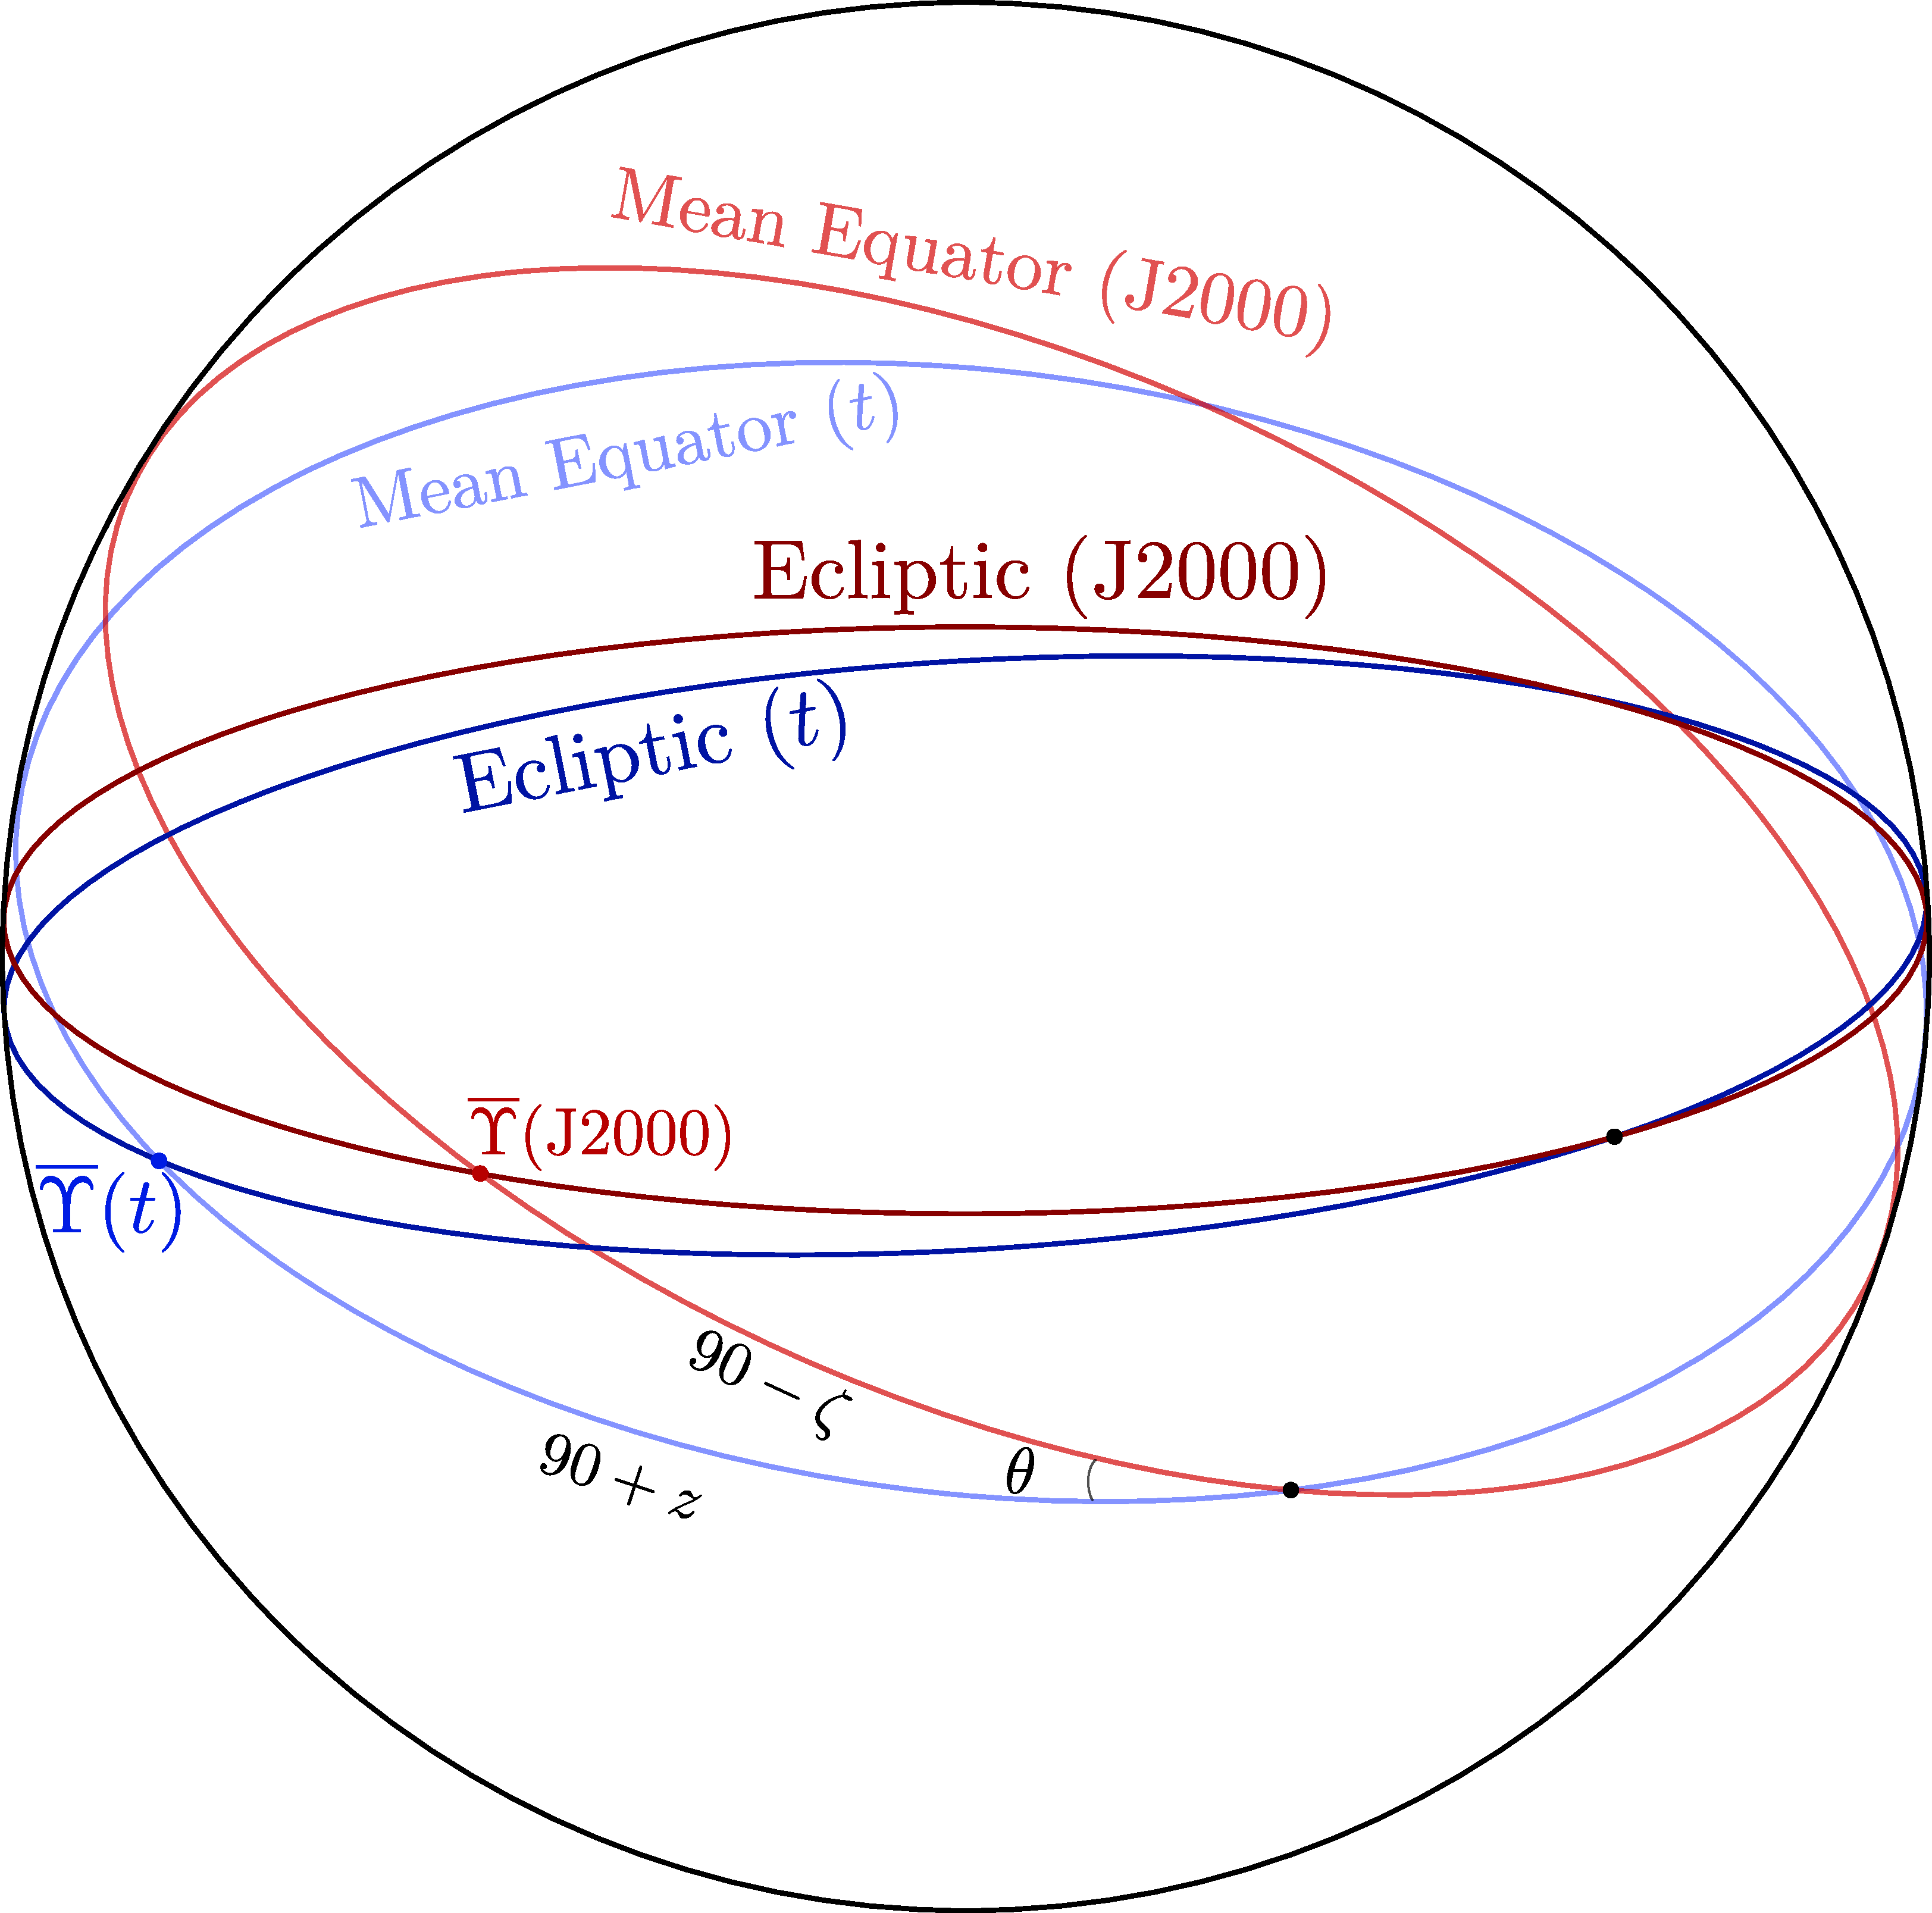
\includegraphics[width=\textwidth]{../Images/ecliptic_equator.pdf}
% \end{minipage}
% \hspace{0.025\textwidth}
% \begin{minipage}[ht]{0.3\textwidth}
% \centering
% 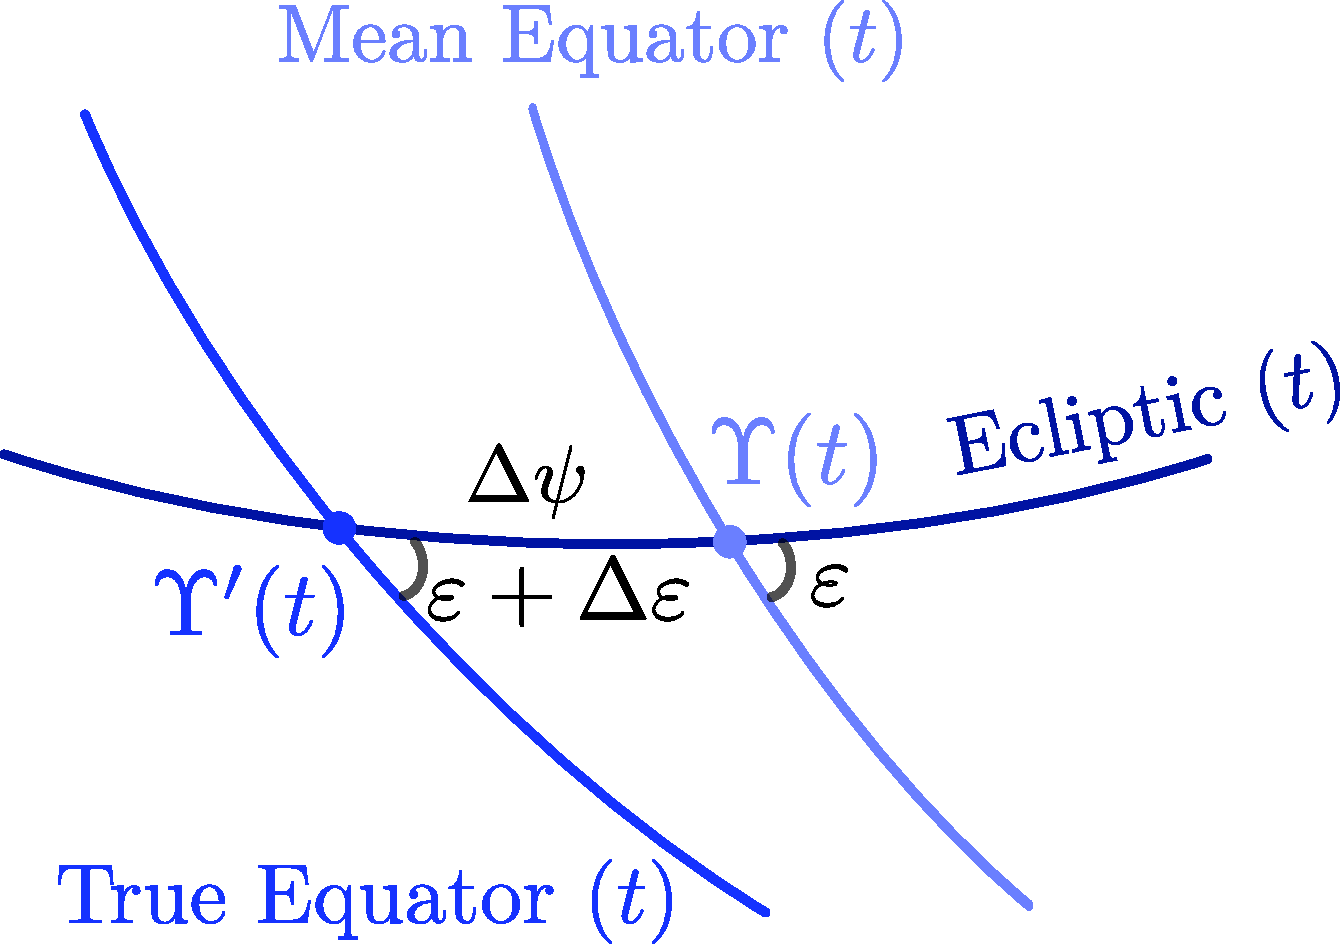
\includegraphics[width=0.9\textwidth]{../Images/nutation_matrix.pdf}
% \end{minipage}
% \hspace{0.025\textwidth}
% \begin{minipage}[ht]{0.3\textwidth}
% \centering
% 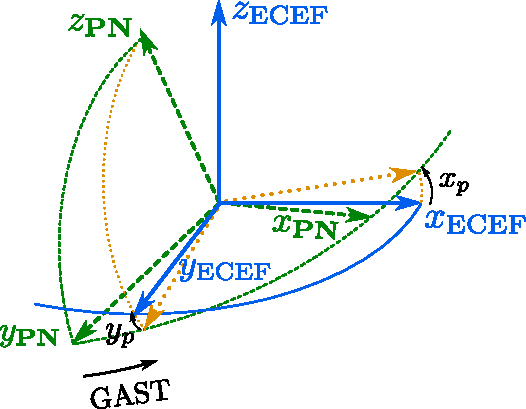
\includegraphics[width=0.9\textwidth]{../Images/polar_motion_matrix.pdf}
% \end{minipage}
% \end{figure}
% \end{frame}
\section{Altres pertorbacions i sistema d'EDOs final}
\begin{frame}
  \frametitle{Altres pertorbacions}
  $\vf{r} = \text{posició del satè\lgem it respecte al centre de masses de la Terra}$

  \vspace{0.25cm}
  \begin{itemize}
    \item<1-> Pertorbacions d'altres cossos (Lluna i Sol):
      $$\frac{GM}{\norm{\vf{s}-\vf{r}}^2}(\vf{s}-\vf{r}) - \frac{GM}{\norm{\vf{s}}^2}\vf{s}$$
    \item<2-> Fregament atmosfèric: $$-\frac{1}{2}C_\mathrm{F} \frac{A}{m}\rho v_\mathrm{rel}\vf{v}_\mathrm{rel}$$
      on $\vf{v}_\mathrm{rel}=\dot{\vf{r}}-\vf{\omega}_\oplus\times\vf{r}$
    \item<3-> Pressió per radiació solar: $$
        -\nu P_\odot C_\mathrm{R} \frac{A_\odot}{m} \frac{\vf{s}_\odot-\vf{r}}{\norm{\vf{s}_\odot-\vf{r}}}
      $$
  \end{itemize}
\end{frame}
\begin{frame}{Sistema d'equacions diferencials ordinàries}
  Utilitzant el mètode de Runge-Kutta-Fehlberg d'ordre 7(8) integrarem el sistema diferencial:
  \begin{equation*}
    \begin{cases}
      \dot{\vf{r}}=\vf{v} \\
      \dot{\vf{v}}=\vf{a}_{\mathrm{GP}} + \delta_{\mathrm{F}}\vf{a}_{\mathrm{F}}+\delta_{\mathrm{R}}\vf{a}_{\mathrm{R}}+\delta_{\mathrm{sol}}\vf{a}_{\mathrm{sol}}+\delta_{\mathrm{lluna}}\vf{a}_\mathrm{lluna}
    \end{cases}
  \end{equation*}
  \pause
  \vspace{0.25cm}

  Les condicions inicials provenen de \textbf{TLEs} (\emph{Two Line Elements sets}).
  \begin{figure}
    \centering
    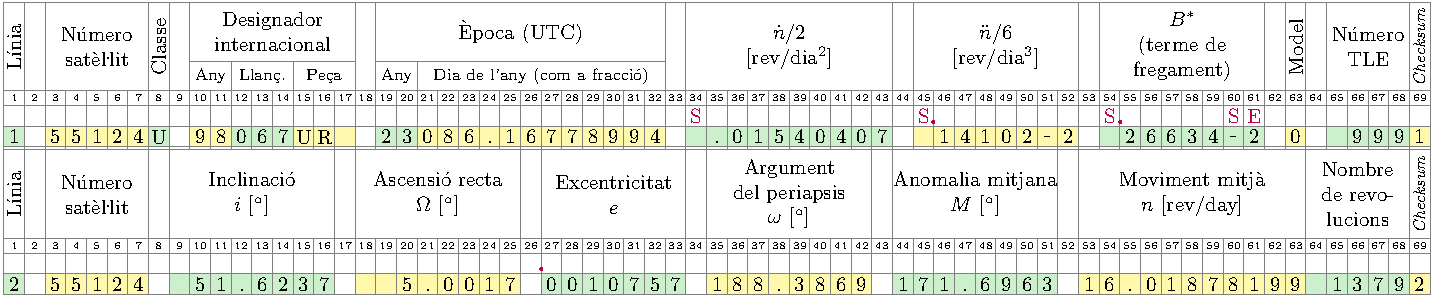
\includegraphics[width=\textwidth]{../Images/TLE_ca.pdf}
  \end{figure}
\end{frame}
\section{Resultats}
\begin{frame}{Resultats - LEO (\emph{Low Earth Orbit})}
  \begin{itemize}
    \item L'ISS fa aproximadament 16 òrbites al dia.
    \item Els satè\lgem its LEO interactuen amb l'atmosfera.
    \item És difícil de predir el fregament atmosfèric.
  \end{itemize}
  \begin{figure}[htbp]
    \centering
    \begin{minipage}[ht]{0.45\textwidth}
      \centering
      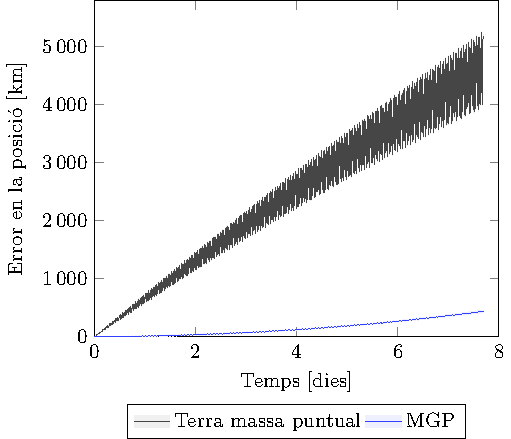
\includegraphics[width=\textwidth]{../Images/simulation/ISS_pointMass_comparison_ca.pdf}
      \caption{\hspace{0.8cm}ISS}
    \end{minipage}
    \hspace{0.0333333\textwidth}
    \begin{minipage}[ht]{0.45\textwidth}
      \centering
      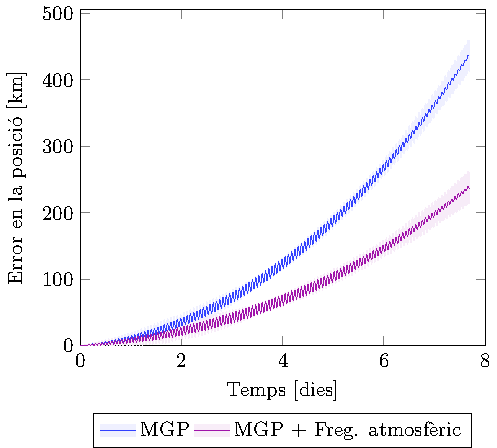
\includegraphics[width=\textwidth]{../Images/simulation/ISS_ca.pdf}
      \caption{\hspace{0.8cm}ISS}
    \end{minipage}
  \end{figure}
\end{frame}
\begin{frame}{Resultats - GEO (\emph{Geostationary Earth Orbit})}
  \begin{minipage}{0.48\textwidth}
    \begin{figure}[ht]
      \centering
      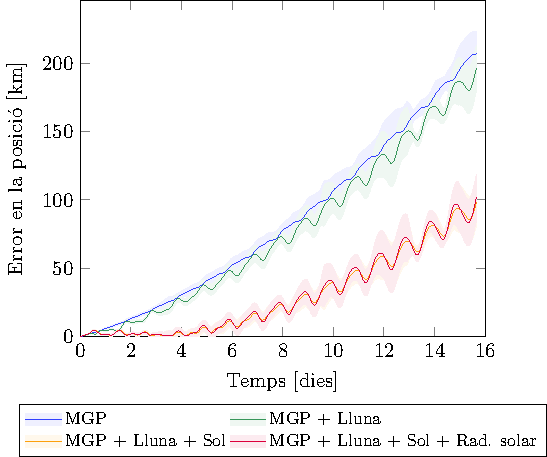
\includegraphics[width=\textwidth]{../Images/simulation/TDRS-3_ca.pdf}
      \caption{TDRS-3}
    \end{figure}
  \end{minipage}
  \hfill
  \begin{minipage}{0.48\textwidth}
    \begin{itemize}
      \item Afegint-hi la Lluna i el Sol, els errors es redueixen.
      \item La pressió per radiació solar augmenta les osci\lgem acions.
      \item Maniobra al voltant del dia 13.
    \end{itemize}
  \end{minipage}
\end{frame}
\section{Conclusions}
\begin{frame}{Conclusions}
  \begin{itemize}
    \item El model de la Terra com a massa puntual no és suficient per predir l'òrbita d'un satè\lgem it durant uns quants dies.
    \item Afegint-hi la Lluna i el Sol, la variabilitat dels errors es redueix.
    \item La pressió per radiació solar n'augmenta les osci\lgem acions.
  \end{itemize}
  \vspace{0.5cm}\pause
  \textbf{Possibles refinaments:}
  \begin{itemize}
    \item Millorar el modelatge del fregament atmosfèric i la pressió per radiació solar.
    \item Estudiar la influència de la inclinació i l'excentricitat en els errors.
  \end{itemize}
\end{frame}
\begin{frame}{Extres}

\end{frame}
\begin{frame}
  Separació de variables: $V=R(r)\Theta(\theta)\Phi(\phi)$
  \begin{gather*}
    \begin{cases}
      \displaystyle\frac{{(r^2R')}'}{R}=n(n+1)                  \\
      \displaystyle\frac{1}{\Theta}\Theta'' =-m^2\vspace{0.1cm} \\
      \displaystyle\frac{\sin\phi}{\Phi}{(\sin\phi\Phi')}'+n(n+1){(\sin\phi)}^2 =m^2
    \end{cases}\!n,m\in\NN\cup{0}, m\leq n
  \end{gather*}\pause
  Imposant condicions de frontera:
  \begin{equation*}
    V =\frac{GM_\oplus}{R_\oplus}\sum_{n=0}^\infty \sum_{m=0}^n{\left(\frac{{R_\oplus}}{r}\right)}^{n+1}(\bar{C}_{n,m}Y_{n,m}^{\mathrm{c}}(\theta,\phi)+\bar{S}_{n,m}Y_{n,m}^{\mathrm{s}}(\theta,\phi))
  \end{equation*}
  on
  \begin{align*}
    Y_{n,m}^{\mathrm{c}}(\theta,\phi) & =N_{n,m}P_{n,m}(\cos\theta)\cos(m\phi) \\
    Y_{n,m}^{\mathrm{s}}(\theta,\phi) & =N_{n,m}P_{n,m}(\cos\theta)\sin(m\phi)
  \end{align*}
  són els \textbf{harmònics esfèrics}.
\end{frame}
\begin{frame}{Esfera celeste}
  \begin{itemize}
    \item Esfera abstracta de radi infinit centrada en la Terra.
    \item Tots els objectes celestes s'hi projecten de forma natural.
  \end{itemize}
  \begin{minipage}{0.45\textwidth}
    \begin{figure}
      \centering
      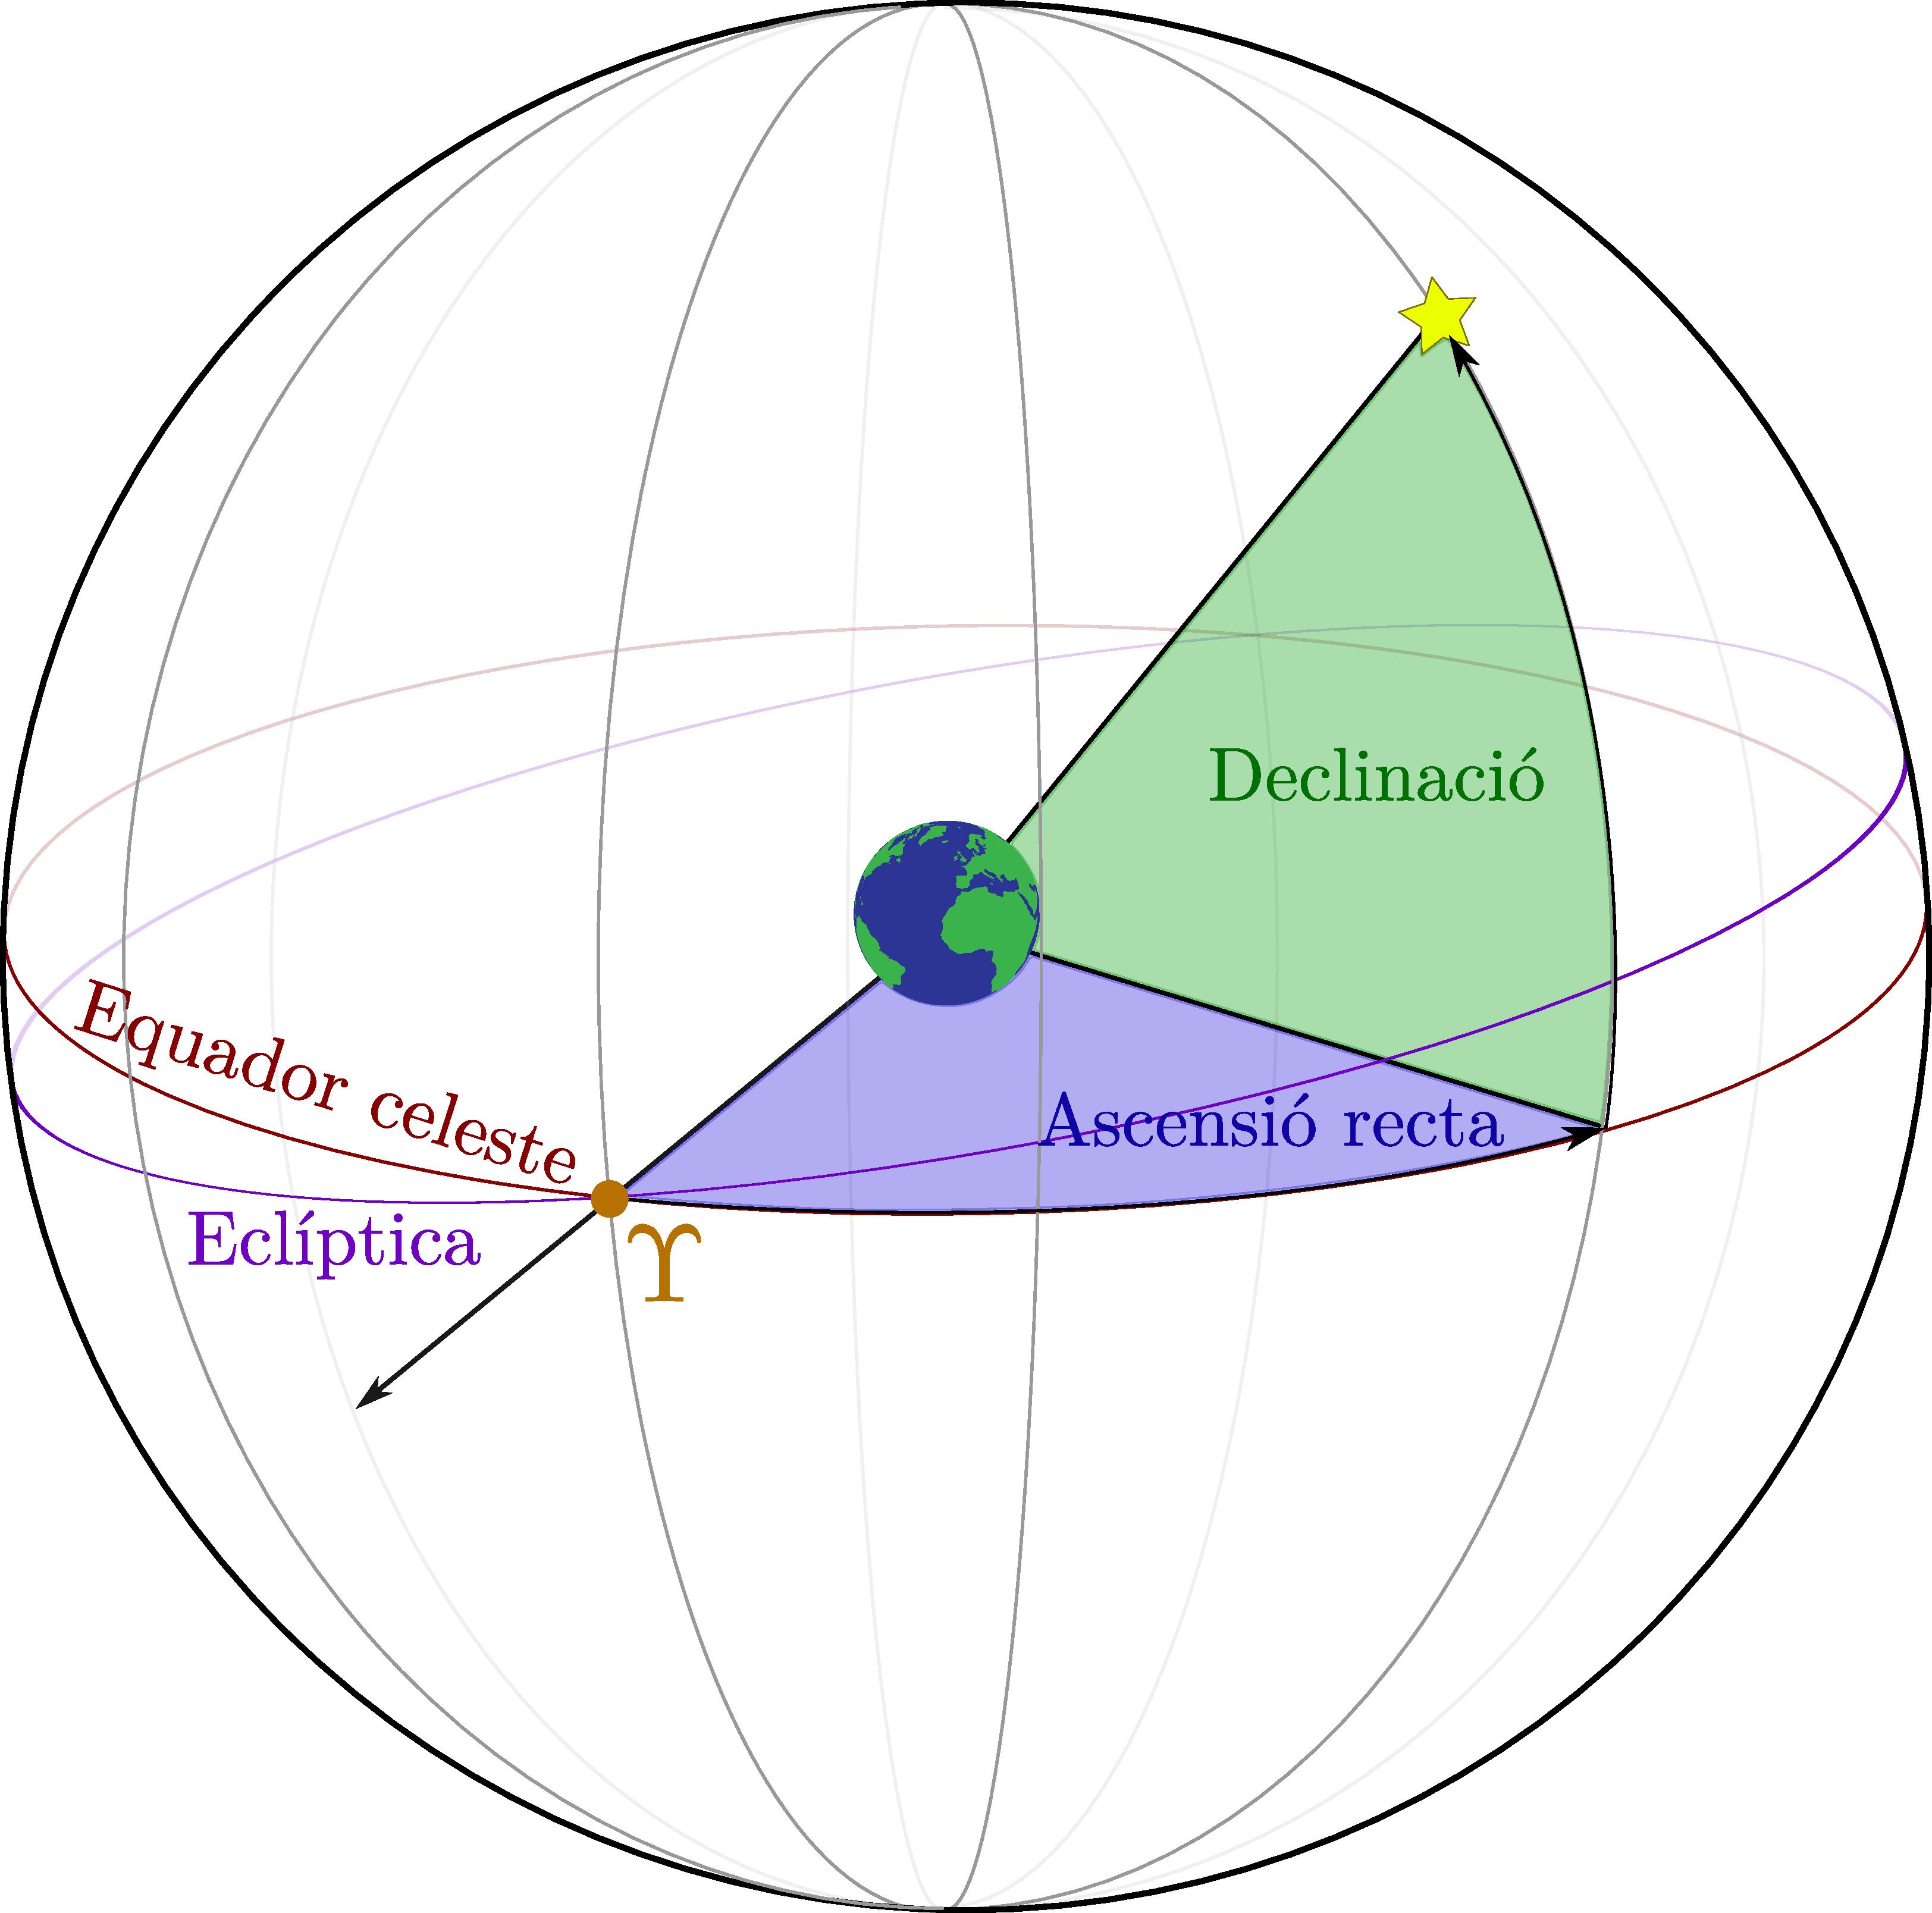
\includegraphics[width=\textwidth]{../Images/right_ascension-decli_ca.pdf}
    \end{figure}
  \end{minipage}\hfill
  \begin{minipage}{0.5\textwidth}
    \textbf{Eix mitjà de rotació:} eix de rotació quan les pertorbacions de nutació es promitgen.

    \textbf{Equador mitjà:} pla perpendicular a l'eix mitjà de rotació.

    \textbf{Equinocci vernal mitjà ($\overline{\Upsilon}$):} el punt d'intersecció entre l'equador mitjà amb l'eclíptica on el Sol creua l'equador celeste de sud a nord.

  \end{minipage}
\end{frame}
\begin{frame}{Sistemes de referència inercials i no inercials}
  Data J2000: 1 de gener de 2000 a les 12:00 TT.
  \vspace{0.5cm}

  \textbf{Quasi-inercial}:
  \begin{itemize}
    \item Eix $x$: apuntant cap a $\overline{\Upsilon}$ de la data J2000
    \item Eix $z$: perpendicular a l'equador mitjà de la data J2000
  \end{itemize}

  \textbf{No inercial} (fix amb la Terra):
  \begin{itemize}
    \item Eix $z$: apuntant cap a l'IRP (\emph{International Reference Pole})
    \item Eix $x$: apuntant cap al meridià zero i situat en el pla perpendicular a l'eix $z$
  \end{itemize}

  En ambdós sistemes, l'eix $y$ s'escull de manera que la base $(x,y,z)$ sigui positiva.
\end{frame}
\begin{frame}{Resultats}
  Esquema de la nostra simulació:
  \begin{figure}
    \centering
    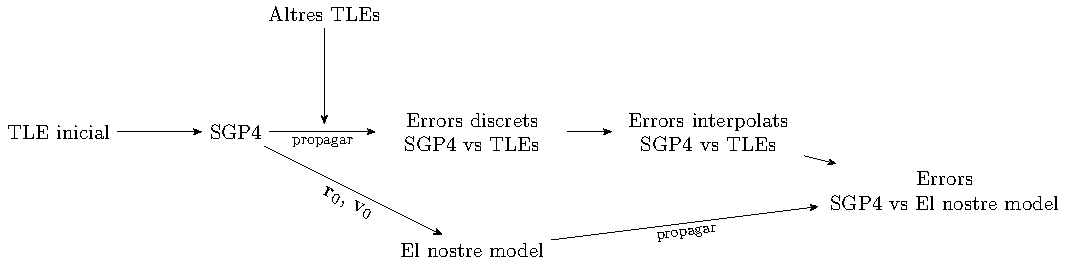
\includegraphics[width=\textwidth]{../Images/simulation_scheme_ca.pdf}
  \end{figure}\pause
  \begin{minipage}{0.4\textwidth}
    \begin{figure}[ht]
      \centering
      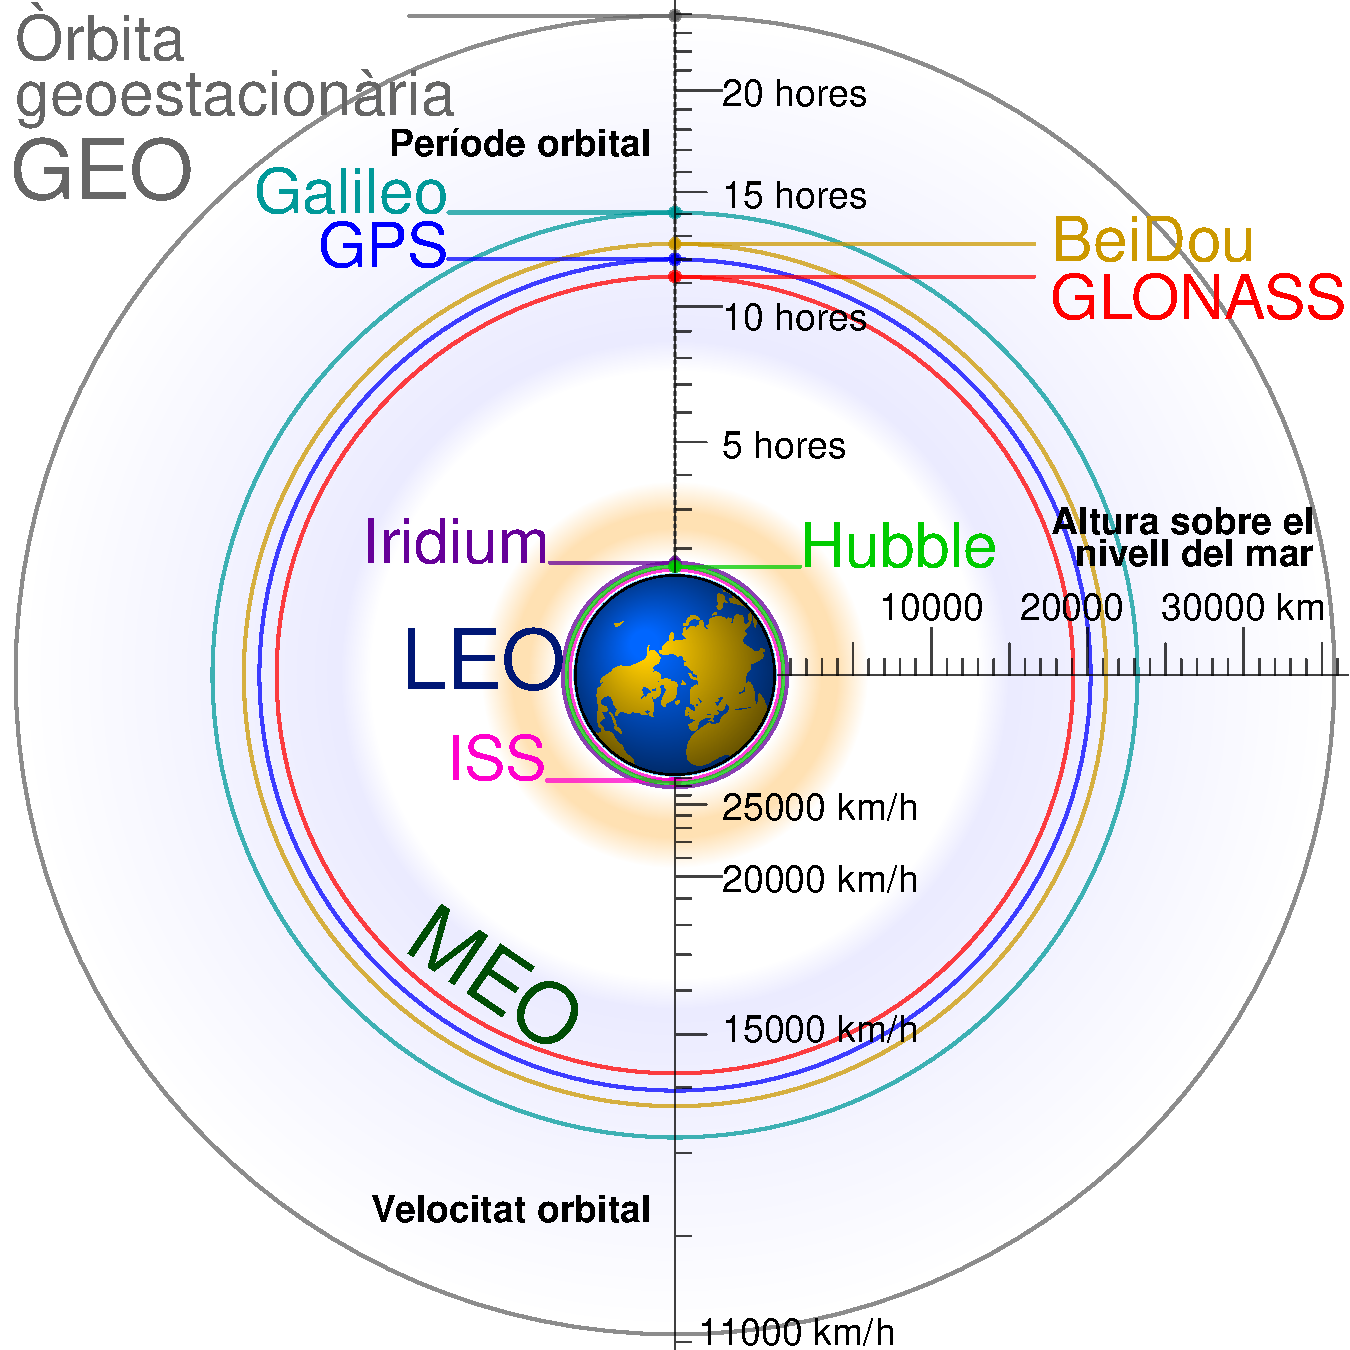
\includegraphics[width=\textwidth]{../Images/satellite_orbits_custom_ca.pdf}
    \end{figure}
  \end{minipage}\hfill
  \begin{minipage}{0.55\textwidth}
    Zones que hem estudiat:
    \begin{itemize}
      \item Satè\lgem its d'òrbita baixa (LEO)
      \item Satè\lgem its d'òrbita mitjana (MEO)
      \item Satè\lgem its d'òrbita geoestacionària (GEO)
    \end{itemize}
  \end{minipage}
\end{frame}
\begin{frame}{Resultats - MEO}
  \begin{figure}[ht]
    \centering
    \begin{minipage}[ht]{0.45\textwidth}
      \centering
      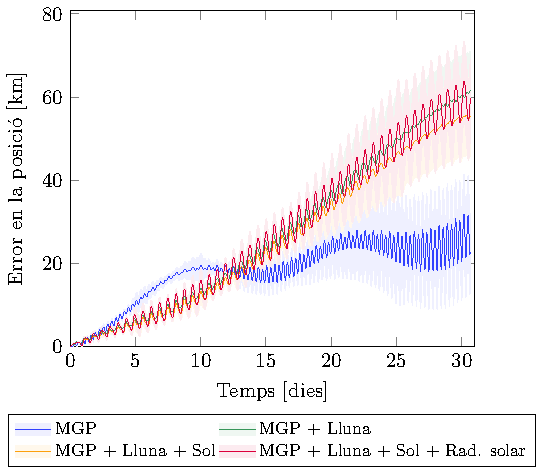
\includegraphics[width=\textwidth]{../Images/simulation/SIRIUS_ca.pdf}
      \caption{Sirius-3}
    \end{minipage}
    \hspace{0.0333333\textwidth}
    \begin{minipage}[ht]{0.45\textwidth}
      \centering
      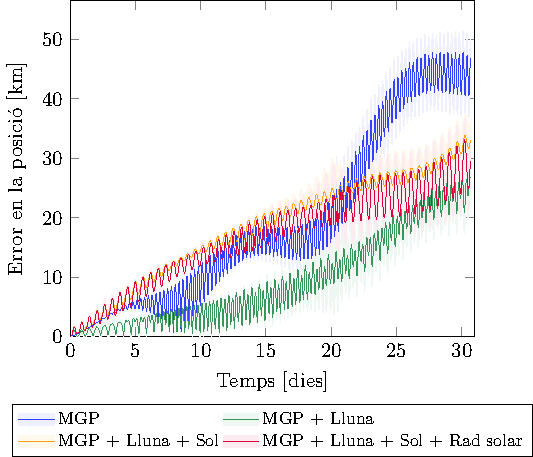
\includegraphics[width=\textwidth]{../Images/simulation/GALILEO_ca.pdf}
      \caption{Galileo-20}
    \end{minipage}
  \end{figure}
  \begin{itemize}
    \item El model geopotential és molt osci\lgem atori.
    \item La Lluna i el Sol redueixen les osci\lgem acions.
    \item La pressió per radiació solar augmenta les osci\lgem acions.
  \end{itemize}
\end{frame}
\end{document}